\section{Shortest Path Trees}

\subsection{Gewichtete Graphen}
\begin{itemize}
    \item jede Kante hat einen assoziierten nummerischen Wert (Gewicht)
    \item z.B. Distanzen, Kosten, etc. repräsentieren
\end{itemize}

\subsection{Kürzester Pfad}
\begin{itemize}
    \item Gegeben sei ein gewichteter Graph mit zwei Vertizes u und v.
    \item Wir möchten den Weg mit dem kleinsten totalen Gewicht zwischen u und v finden
    \item Die Länge des Pfades ist die Summe der Gewichte seiner Kanten
\end{itemize}
\subsubsection{Eigenschaften}
\begin{itemize}
    \item \textbf{Eigenschaft 1:} Ein Teilweg eines kürzesten Weges ist selbst auch ein kürzester Weg
    \item \textbf{Eigenschaft 2:} Es existiert ein Baum von kürzesten Wegen von einem Start-Vertex zu allen anderen Vertizes.
    \item \textbf{Eigenschaft 3:}Baum der kürzesten Wege von Providence
\end{itemize}

\subsection{Dijkstra’s Algorithmus}
\begin{itemize}
    \item Die Distanz eines Vertex v zu einem Vertex s ist die Länge des kürzesten Pfades zwischen s und v
    \item Dijkstra’s Algorithmus berechnet die Distanzen zu allen Vertizes von einem Start-Vertex s aus
\end{itemize}

\subsubsection{Ablauf}
\begin{itemize}
    \item bilden eine Wolke (Cloud) von Vertizes, beginnend mit s und fügen nach und nach alle Vertizes ein
    \item Mit jedem Vertex v speichern wir eine Eigenschaft d(v) welche die Distanz von v zu s im Untergraph (bestehend aus der Wolke und den Nachbar-Vertizes) angibt
    \item Bei jedem Schritt
    \begin{itemize}
        \item fügen der Wolke den Vertex u hinzu, welcher ausserhalb der Wolke ist und die kleinste Distanz d(u) aufweist
        \item aktualisieren die Distanzen von allen Nachbar-Vertizes von u
    \end{itemize}
\end{itemize}

\subsubsection{Laufzeit}
\begin{itemize}
    \item Methode incidentEdges wird für jeden Vertex einmal aufgerufen
    \item Wir setzen/lesen das Distanz- und das Locator-Label eines Vertex z O(deg(z)) mal
    \item Setzen/Lesen eines Labels braucht O(1) Zeit
    \item Jeder Vertex wird einmal in die Priority Queue eingefügt und einmal gelöscht, wobei jedes Einfügen und Löschen O(log n) Zeit benötigt
    \item Der Schlüssel eines Vertex w in der Priority Queue wird maximal deg(w) mal geändert, wobei jede Änderung O(log n) Zeit benötigt
    \item Dijkstra’s Algorithmus läuft in O((n + m) log n) Zeit, vorausgesetzt dass der Graph mit einer Adjazenz-Listen Struktur implementiert ist
\end{itemize}
\subsection{Kanten Relaxation (Entspannung)}
\begin{center}
    \includegraphics[scale=.27]{graphic/15 ShortestPathTrees/Dijkstra’s1.png}
\end{center}
\vspace{-8pt}


\subsubsection{Beispiel}
\begin{center}
    \includegraphics[scale=.25]{graphic/15 ShortestPathTrees/Dijkstra’s2.png}
\end{center}
\vspace{-8pt}

\subsubsection{Algorithmus}
\begin{center}
    \includegraphics[scale=.32]{graphic/15 ShortestPathTrees/Dijkstra’s alg.png}
\end{center}
\vspace{-8pt}

\subsection{Shortes Path Tree}
\begin{center}
    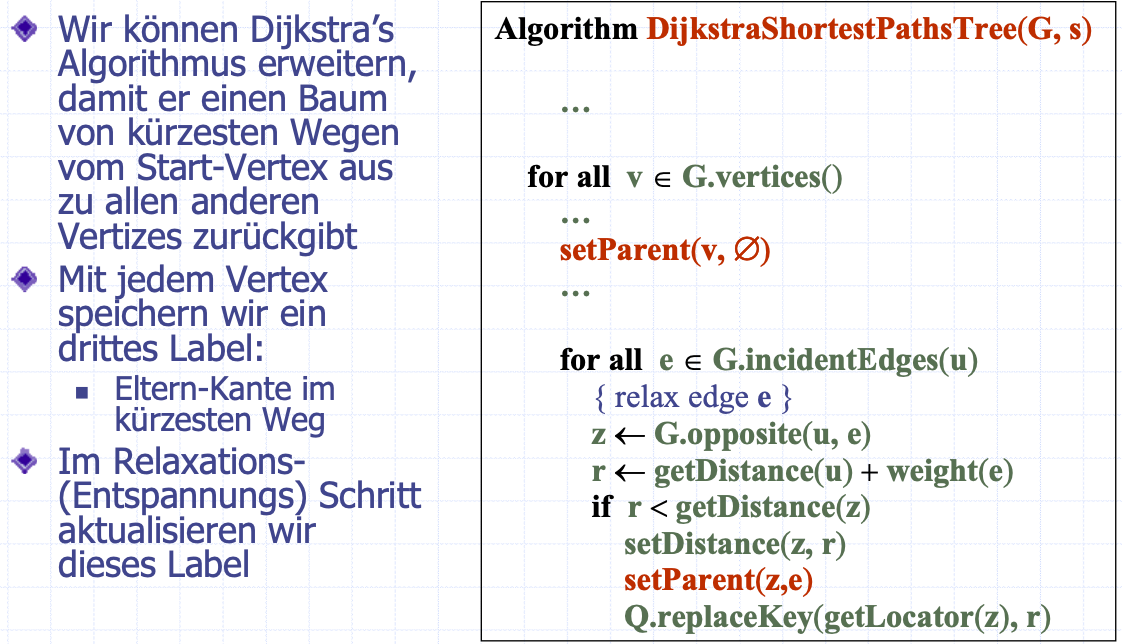
\includegraphics[scale=.3]{graphic/15 ShortestPathTrees/Kürzester Pfad Bäume.png}
\end{center}
\vspace{-8pt}
\subsubsection{Gewichte kleiner Null funktioniert nicht}
\begin{itemize}
    \item Dijkstra’s Algorithmus basiert auf der Greedy (gierig) Methode
    \item Wenn ein Vertex mit einer Kante mit einem Gewicht < 0 später der Wolke hinzugefügt wird, bringt dies die Distanzen für die Vertizes durcheinande
\end{itemize}

\subsection{Bellman-Ford Algorithmus}
\begin{center}
    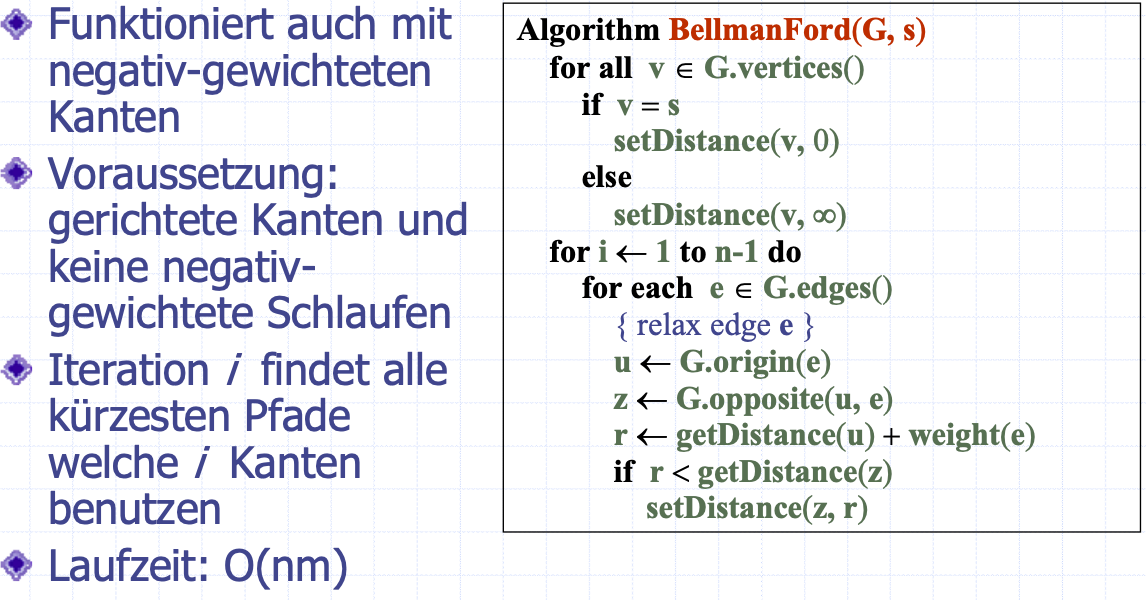
\includegraphics[scale=.25]{graphic/15 ShortestPathTrees/Bellman-Ford1.png}
\end{center}
\vspace{-8pt}
\subsubsection{Beispiel}
\begin{center}
    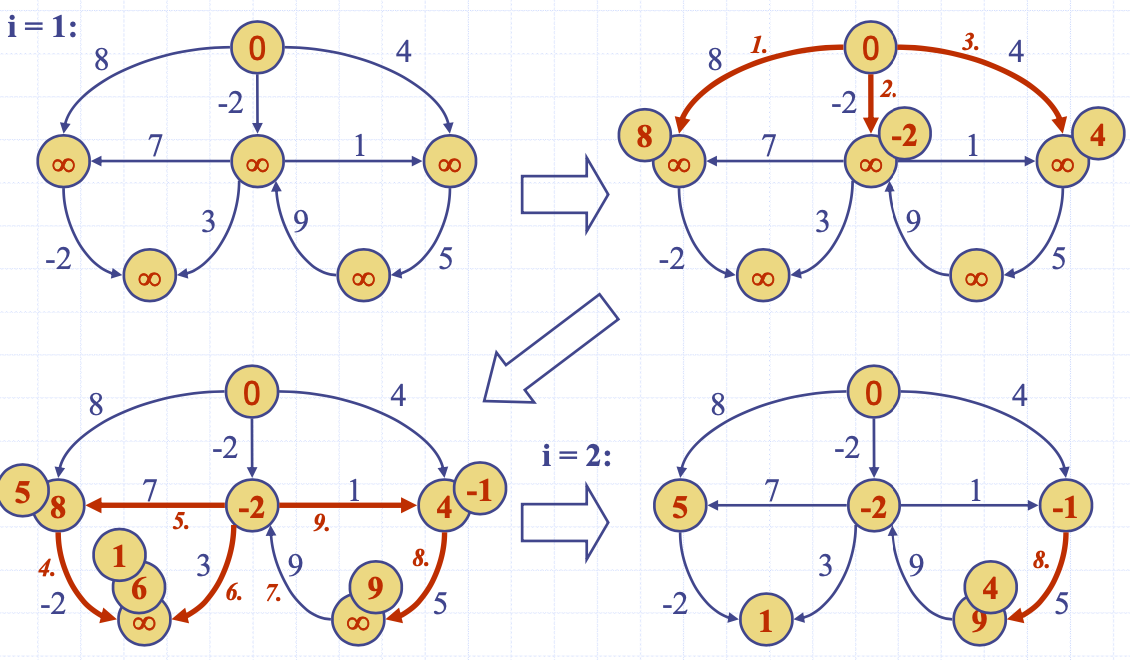
\includegraphics[scale=.25]{graphic/15 ShortestPathTrees/Bellman-Ford2.png}
\end{center}
\vspace{-8pt}

\subsection{DAG-basierter Algorithmus}
\begin{center}
    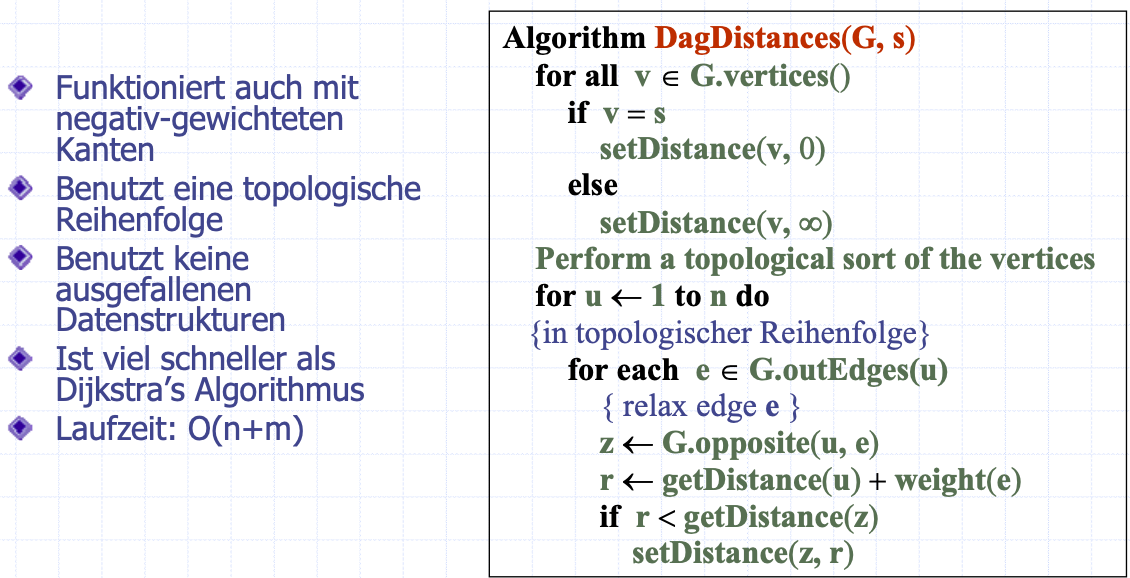
\includegraphics[scale=.32]{graphic/15 ShortestPathTrees/DAG1.png}
\end{center}
\vspace{-8pt}
\subsubsection{Beispiel}
\begin{center}
    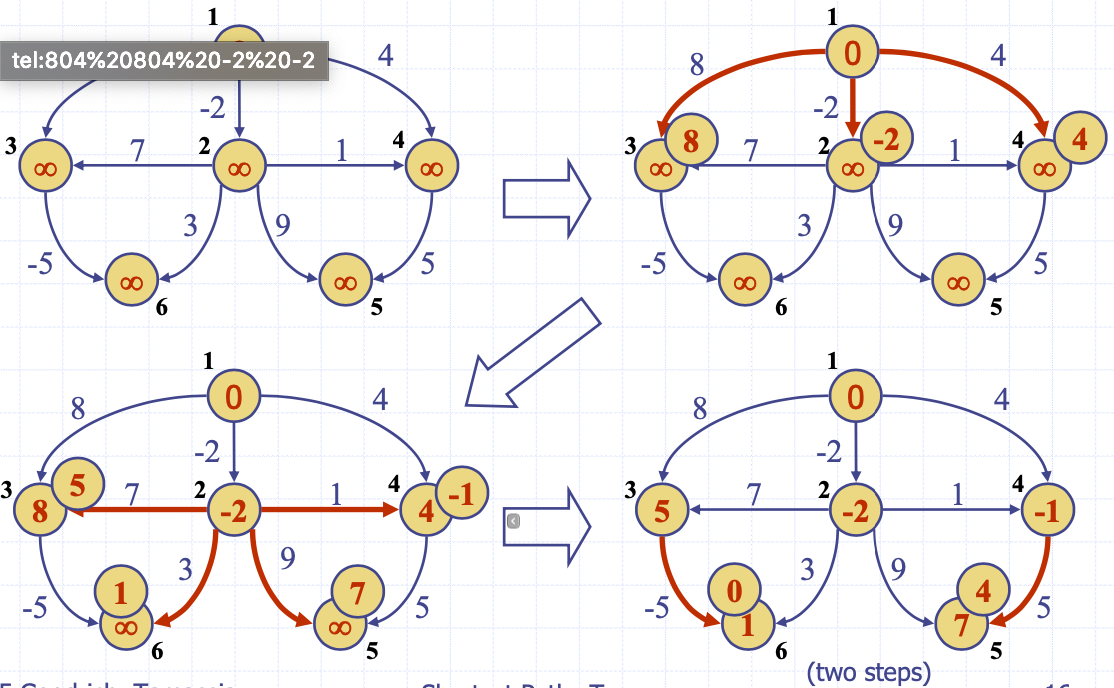
\includegraphics[scale=.3]{graphic/15 ShortestPathTrees/DAG2.png}
\end{center}
\vspace{-8pt}



\newpage